

\chapter{NPUcore-IMPACT特性}
\section{内存管理方面}
\subsection{页表与地址空间管理}

\begin{table}
    \label{tab:addr}
    \centering
    \resizebox{0.7\linewidth}{!}{
\begin{tabular}{|c|c|c|c|}
\hline
地址 & 页号 & 页内偏移 & 总位数 \\
\hline
虚拟地址VA & VPN-38:12 27bit & Offset-11:0 12bit & 39bit \\
物理地址PA & PPN-55:12 44bit & Offset-11:0 12bit & 56bit \\
\hline
\end{tabular}}
\caption{地址详细列表}
\end{table}

在 NPUcore-IMPACT 中,虚拟地址空间和物理地址空间均采用页式管理,且每个页面的大小为 $4KiB (2^{12}B)$。
对于页表以及地址的管理可参见表\autoref{tab:addr}。


\subsection{地址的数据结构抽象}

\begin{lstlisting}[language={rust}, label={code:refill},
        caption={存储地址数据结构}]
#[repr(C)]
#[derive(Copy, Clone, Ord, PartialOrd , Eq, PartialEq)]
pub struct PhysAddr(pub usize);

#[repr(C)]
#[derive(Copy, Clone, Ord, PartialOrd , Eq, PartialEq)]
pub struct VirtAddr(pub usize);

#[repr(C)]
#[derive(Copy, Clone, Ord, PartialOrd , Eq, PartialEq)]
pub struct PhysPageNum(pub usize);

#[repr(C)]
#[derive(Copy, Clone, Ord, PartialOrd , Eq, PartialEq)]
pub struct VirtPageNum(pub usize);
\end{lstlisting}
上面分别给出了物理地址 PA、虚拟地址 VA、物理页号 PPN、虚拟页号 VPN 的类型声明,它们都是元组式结构体,可以看成 usize 的一种简单包装。我们刻意将它们各自抽象出不同的类型而不是都使用与 RISC-V 64 硬件直接对应的 usize 基本类型,是为了在 Rust 编译器的帮助下,通过多种安全且方便的类型转换来构建页表.

\subsection{页表项}

\begin{figure}[h]
    \centering
    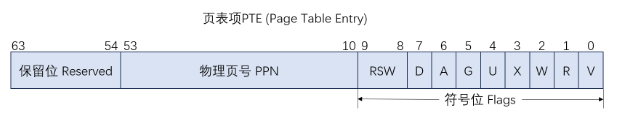
\includegraphics[width=1\linewidth]{figs/PTE.PNG}
    \caption{页表项的格式}
    \label{P}
\end{figure}

其中,对于符号位的详细解释如下:
\begin{itemize}
    \item V(Valid):有效位。仅当 V 为 1 时,该页表项合法;
    \item R(Read)/W(Write)/X(eXecute):分别表示索引到这个页表项的对应虚拟页面是否允许读/写/执行;
    \item U(User):表示索引到这个页表项的对应虚拟页面是否在 CPU 处于 U 特权级的情况下允许访问;
    \item G(Global):全局标志。为 1 时表明该页面为全局页面;
    \item A(Accessed):处理器使用此位来记录自页表项上的这一位被清零后,其对应虚拟页面是否被访问过;
    \item D(Dirty):处理器使用此位来记录自页表项上的这一位被清零后,其对应虚拟页面是否被修改过;
    \item RSW(Reserved for Supervisor softWare):保留位。该部分被处理器忽略,软件可以使用。
\end{itemize}

\subsection{地址空间}
内核地址空间有四个标志位,具体为\textit{R - 读;W - 写;X - 执行;U - 用户。}

\textit{对于内核程序区域而言:}

在\textbf{os/src/linker.in.ld}下,我们可以找到对应的基址,其值为:\textbf{0x0000000090000000}。
而对于本次新的开发板LoongArch-2K1000而言,其MMIO区域并无多少设备,仅有一UART寄存器,具体可在\textbf{os/src/arch/la64/board/2k1000.rs}下找到UART寄存器地址:\textbf{0x1fe20000}.


目前仅介绍了部分重要地址,由于更换开发板,大部分地址常数已经重写,具体可参见\textbf{os/src/arch/la64/config.rs}。
\begin{lstlisting}[language={rust}, label={code:config},
    caption={os/src/arch/la64/config.rs}]
pub const MEMORY_SIZE: usize = 0x1000_0000;
pub const USER_STACK_SIZE: usize = PAGE_SIZE * 40;
pub const USER_HEAP_SIZE: usize = PAGE_SIZE * 20;
pub const SYSTEM_TASK_LIMIT: usize = 128;
pub const DEFAULT_FD_LIMIT: usize = 128;
pub const SYSTEM_FD_LIMIT: usize = 256;
pub const PAGE_SIZE: usize = 0x1000;
pub const PAGE_SIZE_BITS: usize = PAGE_SIZE.trailing_zeros() as usize;
pub const PTE_WIDTH: usize = 8;
pub const PTE_WIDTH_BITS: usize = PTE_WIDTH.trailing_zeros() as usize;
pub const DIR_WIDTH: usize = PAGE_SIZE_BITS - PTE_WIDTH_BITS;
pub const DIRTY_WIDTH: usize = 0x100_0000;
#[cfg(debug_assertions)]
pub const KSTACK_PG_NUM_SHIFT: usize = 16usize.trailing_zeros() as usize;
#[cfg(not(debug_assertions))]
pub const KSTACK_PG_NUM_SHIFT: usize = 2usize.trailing_zeros() as usize;

pub const KERNEL_STACK_SIZE: usize = PAGE_SIZE << KSTACK_PG_NUM_SHIFT;
pub const KERNEL_HEAP_SIZE: usize = PAGE_SIZE * 0x3000;

// Addresses
/// Maximum length of a physical address
pub const PALEN: usize = 48;
/// Maximum length of a virtual address
pub const VALEN: usize = 48;
/// Maximum address in virtual address space.
/// May be used to extract virtual address from a segmented address
/// '0'-extension may be performed using this mask.
pub const VA_MASK: usize = (1 << VALEN) - 1;
/// Mask for extracting segment number from usize address.
/// '1'-extension may be performed using this mask.
/// e.g. 'flag' |= 'SEG_MASK'
pub const SEG_MASK: usize = !VA_MASK;
/// Mask for extracting segment number from VPN.
/// All-one for segment field.
/// '1'-extension may be performed using this mask.
/// e.g. 'flag' |= 'SEG_MASK'
pub const VPN_SEG_MASK: usize = SEG_MASK >> PAGE_SIZE_BITS;

pub const HIGH_BASE_EIGHT: usize = 0x8000_0000_0000_0000;
pub const HIGH_BASE_ZERO: usize = 0x0000_0000_0000_0000;

// manually make usable memory space equal
pub const SUC_DMW_VESG: usize = 8;
pub const MEMORY_HIGH_BASE: usize = HIGH_BASE_ZERO;
pub const MEMORY_HIGH_BASE_VPN: usize = MEMORY_HIGH_BASE >> PAGE_SIZE_BITS;
pub const USER_STACK_BASE: usize = TASK_SIZE - PAGE_SIZE | LA_START;
pub const MEMORY_START: usize = 0x0000_0000_9000_0000;
pub const MEMORY_END: usize = MEMORY_SIZE + MEMORY_START;

pub const SV39_SPACE: usize = 1 << 39;
pub const USR_SPACE_LEN: usize = SV39_SPACE >> 2;
pub const LA_START: usize = 0x1_2000_0000;
pub const USR_VIRT_SPACE_END: usize = USR_SPACE_LEN - 1;
pub const TRAMPOLINE: usize = SIGNAL_TRAMPOLINE; // The trampoline is NOT mapped in LA.
pub const SIGNAL_TRAMPOLINE: usize = USR_VIRT_SPACE_END - PAGE_SIZE + 1;
pub const TRAP_CONTEXT_BASE: usize = SIGNAL_TRAMPOLINE - PAGE_SIZE;
pub const USR_MMAP_END: usize = TRAP_CONTEXT_BASE - PAGE_SIZE;
pub const USR_MMAP_BASE: usize = USR_MMAP_END - USR_SPACE_LEN / 8 + 0x3000;
pub const TASK_SIZE: usize = USR_MMAP_BASE - USR_SPACE_LEN / 8;
pub const ELF_DYN_BASE: usize = (((TASK_SIZE - LA_START) / 3 * 2) | LA_START) \& (!(PAGE_SIZE - 1));

pub const MMAP_BASE: usize = 0xFFFF_FF80_0000_0000;
pub const MMAP_END: usize = 0xFFFF_FFFF_FFFF_0000;
pub const SKIP_NUM: usize = 1;

pub const DISK_IMAGE_BASE: usize = 0x800_0000 + MEMORY_START;
pub const BUFFER_CACHE_NUM: usize = 256 * 1024 * 1024 / 2048 * 4 / 2048;

pub static mut CLOCK_FREQ: usize = 0;
\end{lstlisting}


\section{进程调度方面}
对于进程调度,NPUcore-IMPACT给出了一系列方法用于提升操作系统的性能。

\begin{figure}
    \centering
    \label{fig:pro}
    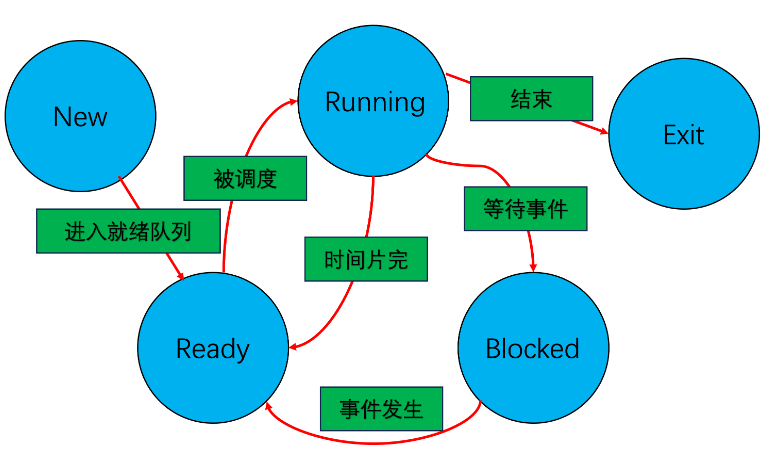
\includegraphics[width=1\linewidth]{figs/Proc.PNG}
    \caption{进程生命周期示意图}
\end{figure}

\subsection{进程生命周期}
对于NPUcore-IMPACT的进程生命周期,我们给出\autoref{fig:pro}以有直观理解
团队在进行性能优化时,发现在操作系统运行示例程序时,
IO操作导致CPU挂起的性能损失非常之大,因此我们将调度器进行了大改(如\autoref{tab:复用}),
使其完全支持了阻塞式的进程调度模式,即构建挂起队列,使进程不能获得资源时可被挂起,直到满足可操作的条件后再进行操作。。
\begin{table}
    \centering
    \label{tab:复用}
    \resizebox{\linewidth}{!}{
\begin{tabular}{|c|c|}
    \hline
    单核/多核 & 单核 \\
    \hline
    资源复用思路 & 一段所有进程共享的跳板代码$+$一个进程的私有的保存现场的帧\\
    资源回收思路 & 释放一部分资源等待父进程完成剩下资源回收\\
    \hline
    进程管理方式 & TCB* \\
    \hline
\end{tabular}}
\caption{NPUcore-IMPACT的复用思路}
\end{table}



\subsection{资源复用}
这里引出我们内核特殊的一点,即使用TCB(TaskControlBlock/任务控制块)(如下面展示的TCB结构体代码)来代替传统的 PCB 数据结构,我们
将线程视为共享栈的进程。
\begin{lstlisting}[language={rust}, label={code:refill},
        caption={TCB结构体}]
pub struct TaskControlBlock {
    // immutable
    pub pid: PidHandle ,
    pub tid: usize,
    pub tgid: usize,
    pub kstack: KernelStack ,
    pub ustack_base: usize,
    pub exit_signal: Signals ,
    // mutable
    inner: Mutex<TaskControlBlockInner >,
    // shareable and mutable
    pub exe: Arc<Mutex<FileDescriptor >>,
    pub tid_allocator: Arc<Mutex<RecycleAllocator >>,
    pub files: Arc<Mutex<FdTable >>,
    pub fs: Arc<Mutex<FsStatus >>,
    pub vm: Arc<Mutex<MemorySet >>,
    pub sighand: Arc<Mutex<Vec<Option<Box<SigAction >>>>>,
    pub futex: Arc<Mutex<Futex>>,
}
\end{lstlisting}


\begin{figure}[h]
    \centering
    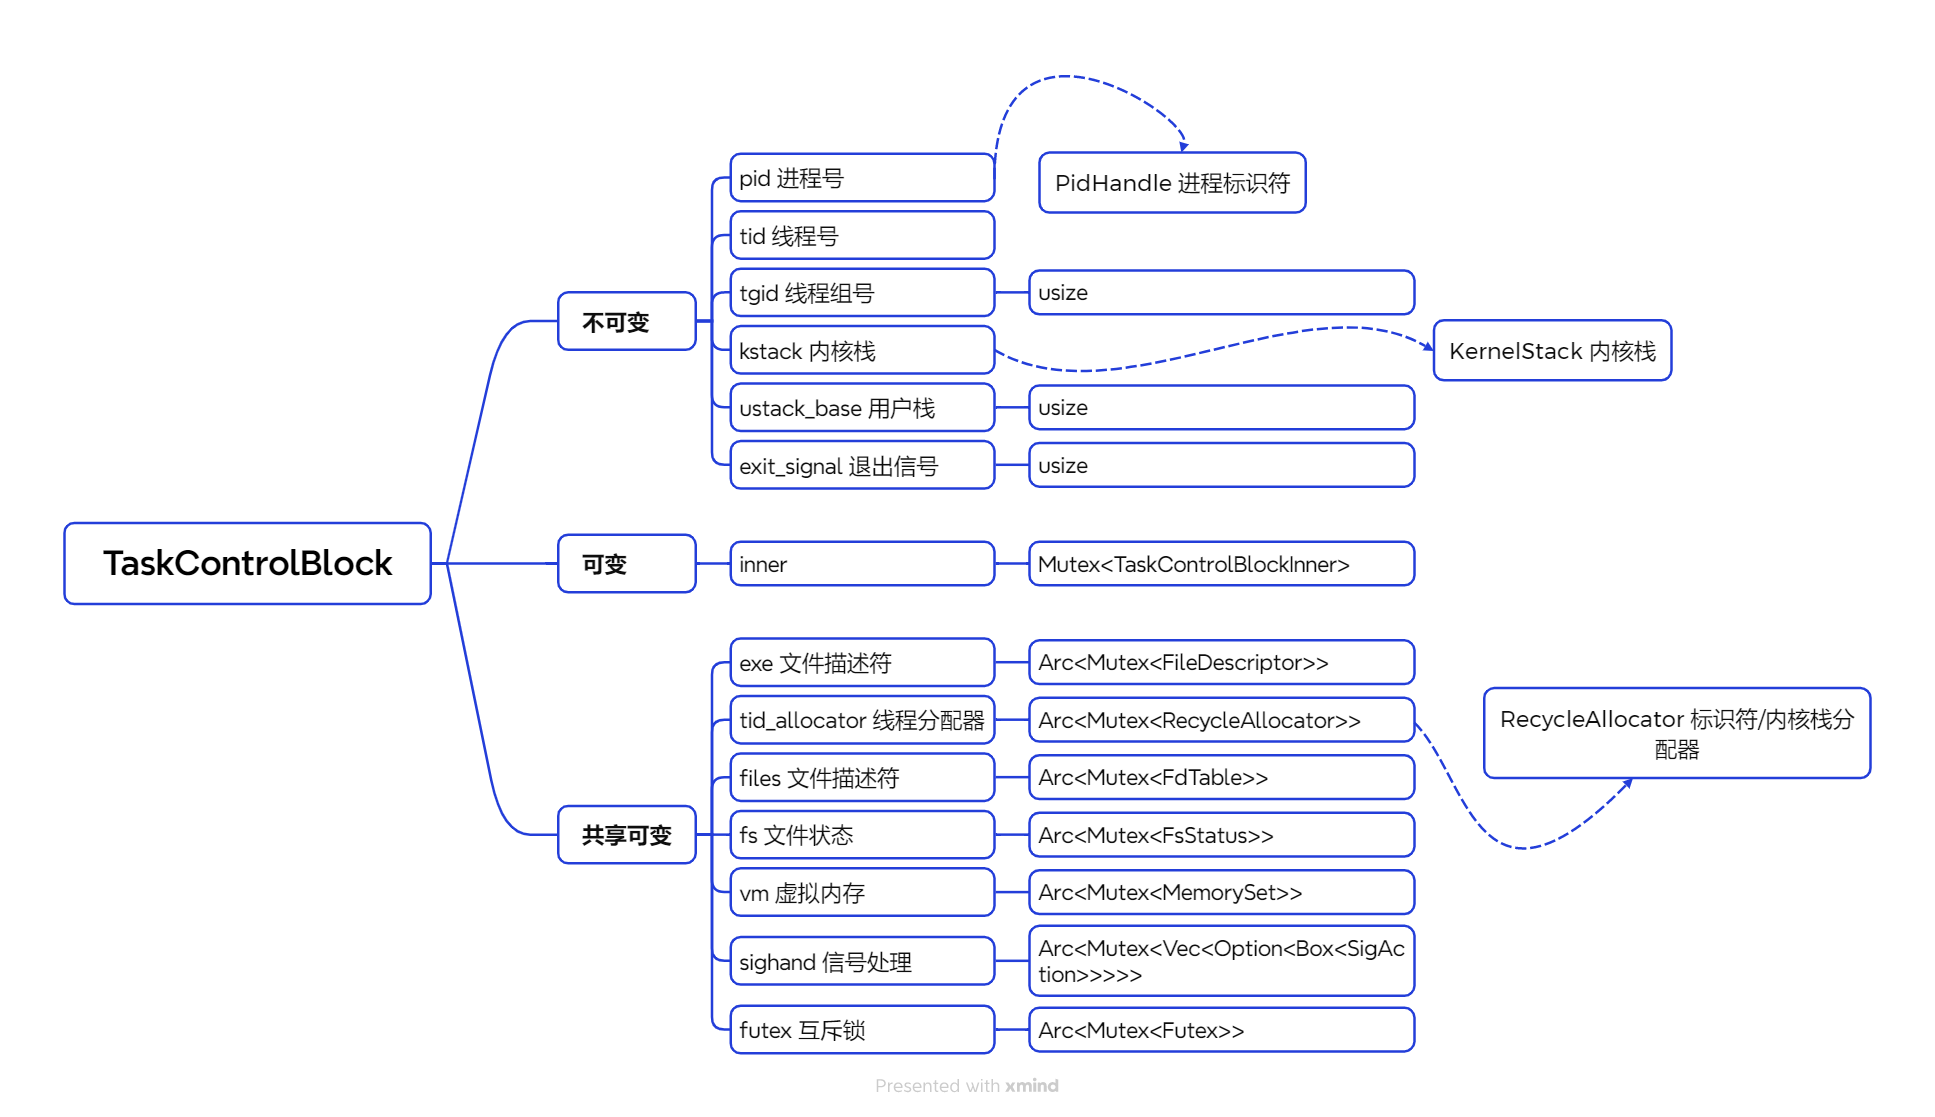
\includegraphics[width=1\linewidth]{figs/TCBBlock.png}
    \caption{TCB结构示意图}
    \label{TCB结构示意图}
\end{figure}

如上述定义的TCB,使得线程在内核中的理解,变为了这样一个可以与同线程组tgid共享内存空间的进程即为线程。

\section{文件系统方面}

目前来讲,NPUcore-IMPACT已经完美支持了 fat32 文件系统,但因耦合度较高,目前我们正在进行解耦合操作,且会在后面支持 ext4 文件系统靠拢。
对于 fat32 文件系统,是我们先前 NPUcore 的增量,不属于我们团队的贡献,因此这里不再赘述,仅在下面给出NPUcore-IMPACT的具体参数。

\subsection{fat32 具体参数}

fat32文件系统是个较为简单的系统,当然,其系统的易移植特性与其简单耐用的特性使其成为了几乎所有系统在初始阶段的第一选择。对于NPUcore-IMPACT,我们可以用一个简单的示意图\ref{fig:fs}来描述他

\begin{figure}[htb]
    \centering
    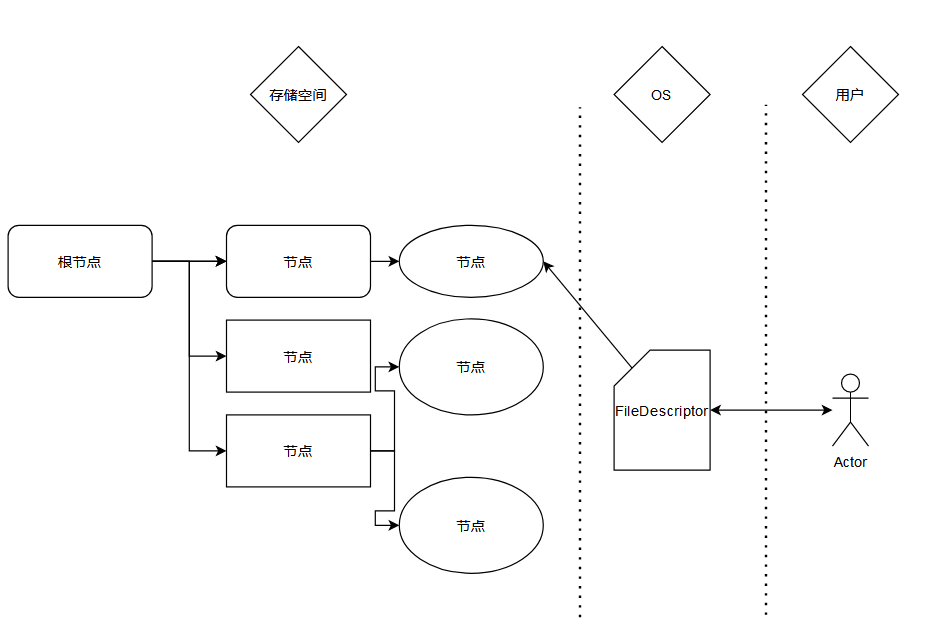
\includegraphics[width=1\linewidth]{figs/dirt.PNG}
    \label{fig:fs}
    \caption{NPUcore-IMPACT的文件系统示意图}
\end{figure}

\subsubsection{FileDescriptor}

如果用简单的描述来简述NPUcore-IMPACT的文件系统,那可以将之理解为一栋楼,我们利用一个描述每个房间的FileDescriptor类的指针来读取一个文件的信息,可以毫不为过的将其理解为我们的文件类型指针, \textbf{FileDescriptor的具体定义如下所示:}

\begin{lstlisting}[language={rust}, label={code:refill}, caption={FileDescriptor}]
    //fs/mod.rs
    #[derive(Clone)]
    pub struct FileDescriptor {
        cloexec: bool,
        nonblock: bool,
        pub file: Arc<dyn File>,
    }
\end{lstlisting}

\subsubsection{文件树结构}

以下是我们定义文件树节点的结构体:

\begin{lstlisting}[language={rust}, label={code:refill}, caption={FileDescriptor}]
    pub struct DirectoryTreeNode {
        /// If this is a directory
        /// 1. cwd
        /// 2. mount point
        /// 3. root node
        /// If this is a file
        /// 1. executed by some processes
        /// This parameter will add 1 when opening
        spe_usage: Mutex<usize>,
        name: String,
        filesystem: Arc<FileSystem>,
        file: Arc<dyn File>,
        selfptr: Mutex<Weak<Self>>,
        father: Mutex<Weak<Self>>,
        children: RwLock<Option<BTreeMap<String, Arc<Self>>>>,
    }
\end{lstlisting}

在通过文件树寻找制定文件的过程中,首先会判断文件的路径前缀是否在路径缓存
中,这样使大量文件操作效率更高,同时 NPUcore 也对一些默认的路径进行了路径的
转化,这部分将于后续5.4中详细说明。

\subsection{NPUcore-IMPACT BitFlags一览}

我们遵循原版POSIX的flag编码,源码如下:
\begin{lstlisting}[language={rust}, label={code:refill}, caption={FileDescriptor}]
    bitflags! {
        pub struct OpenFlags: u32 {
            const O_RDONLY      =   0o0;
            const O_WRONLY      =   0o1;
            const O_RDWR        =   0o2;

            const O_CREAT       =   0o100;
            const O_EXCL        =   0o200;
            const O_NOCTTY      =   0o400;
            const O_TRUNC       =   0o1000;

            const O_APPEND      =   0o2000;
            const O_NONBLOCK    =   0o4000;
            const O_DSYNC       =   0o10000;
            const O_SYNC        =   0o4010000;
            const O_RSYNC       =   0o4010000;
            const O_DIRECTORY   =   0o200000;
            const O_NOFOLLOW    =   0o400000;
            const O_CLOEXEC     =   0o2000000;
            const O_ASYNC       =   0o20000;
            const O_DIRECT      =   0o40000;
            const O_LARGEFILE   =   0o100000;
            const O_NOATIME     =   0o1000000;
            const O_PATH        =   0o10000000;
            const O_TMPFILE     =   0o20200000;
        }
    }

    bitflags! {
        pub struct SeekWhence: u32 {
            const SEEK_SET  =   0; /* set to offset bytes.  */
            const SEEK_CUR  =   1; /* set to its current location plus offset bytes.  */
            const SEEK_END  =   2; /* set to the size of the file plus offset bytes.  */
        }
    }

    bitflags! {
        pub struct StatMode: u32 {
            ///bit mask for the file type bit field
            const S_IFMT    =   0o170000;
            ///socket
            const S_IFSOCK  =   0o140000;
            ///symbolic link
            const S_IFLNK   =   0o120000;
            ///regular file
            const S_IFREG   =   0o100000;
            ///block device
            const S_IFBLK   =   0o060000;
            ///directory
            const S_IFDIR   =   0o040000;
            ///character device
            const S_IFCHR   =   0o020000;
            ///FIFO
            const S_IFIFO   =   0o010000;

            ///set-user-ID bit (see execve(2))
            const S_ISUID   =   0o4000;
            ///set-group-ID bit (see below)
            const S_ISGID   =   0o2000;
            ///sticky bit (see below)
            const S_ISVTX   =   0o1000;

            ///owner has read, write, and execute permission
            const S_IRWXU   =   0o0700;
            ///owner has read permission
            const S_IRUSR   =   0o0400;
            ///owner has write permission
            const S_IWUSR   =   0o0200;
            ///owner has execute permission
            const S_IXUSR   =   0o0100;

            ///group has read, write, and execute permission
            const S_IRWXG   =   0o0070;
            ///group has read permission
            const S_IRGRP   =   0o0040;
            ///group has write permission
            const S_IWGRP   =   0o0020;
            ///group has execute permission
            const S_IXGRP   =   0o0010;

            ///others (not in group) have read, write,and execute permission
            const S_IRWXO   =   0o0007;
            ///others have read permission
            const S_IROTH   =   0o0004;
            ///others have write permission
            const S_IWOTH   =   0o0002;
            ///others have execute permission
            const S_IXOTH   =   0o0001;
        }
    }
\end{lstlisting}

\subsection{NPUcore-IMPACT的目标与计划}

目前我们对于NPUcore-IMPACT整体的性能指标感到较为满意,但并不满足于功能较为单一的现状,目前我们正在为NPUcore-IMPACT添加更多的功能。
由于现在的存储设备技术发展迅速,存储单元的价格已经出现了大幅度下降。同时,随着芯片技术发展,计算机性能变得更加强劲,文件大小也跟着变大,fat32仅能满足\textbf{最大4GB}的单文件存储能力已经远远无法支持新一代设备了,所以我们计划为其添加ext4文件系统支持。
同时由于网络层对于文件系统的依赖耦合程度较高\textit{(Unix_Like系统大多依赖VFS来对设备进行控制,即把设备当做一个可以进行读写的类管道文件)},我们暂时放弃了已经写好的fat32下的网络支持,计划于ext4完成适配再进行添加。最终我们拟定在决赛时提交完整版文件系统。